\documentclass[fleqn]{article}
\usepackage{amsmath}    % math equation environments
\usepackage{amssymb}    % math symbols such as natural numbers N.
\usepackage{graphicx}

\newenvironment{answers}{ % same as enumerate but with more space between each answer
	\begin{enumerate}
		\setlength{\itemsep}{\bigskipamount}
}{\end{enumerate}}

\newcommand\Item[1][]{ % custom \Item command for block math
  \ifx\relax#1\relax  \item \else \item[#1] \fi
  \abovedisplayskip=0pt\abovedisplayshortskip=0pt~\vspace*{-\baselineskip}}

% paragraph indentation within enumerations
\usepackage{enumitem}
\setlist{parsep=4pt,listparindent=\parindent}

\title{Linear Algebra 2 \\
\medskip
\large Homework 1.5 -- Roots of Unity}
\author{Abraham Murciano}

\begin{document}

\maketitle

\begin{answers}

	\item
		\begin{enumerate}
			\item
				If \(z\) is a root of the equation \(x^8 = 1\), then it is not necessarily true that \(\operatorname{Re}(z) > 0\), since as shown in figure \ref{roots-of-unity-8}, this is only true for the three rightmost of the eight roots.
				\begin{figure}[htbp]
					\centering
					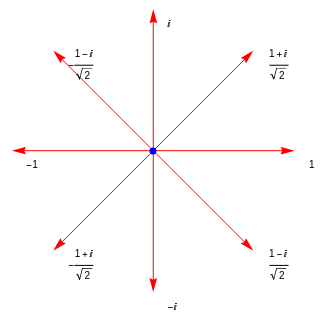
\includegraphics{roots-of-unity-8.png}
					\caption{The roots of unity of order 8.}
					\label{roots-of-unity-8}
				\end{figure}

			\item
				If \(z\) is a root of the equation \(x^6 = 1\), then it is not guaranteed to be the case that \(\operatorname{Im}(z) \neq 0\), since as is visible in figure \ref{roots-of-unity-6}, there are in fact two real solutions, namely 1 and \(-1\).
				\begin{figure}[htbp]
					\centering
					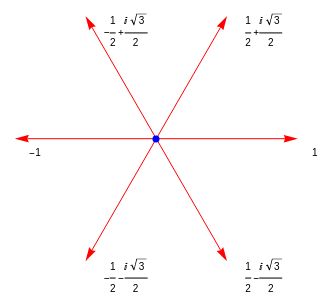
\includegraphics{roots-of-unity-6.png}
					\caption{The roots of unity of order 6.}
					\label{roots-of-unity-6}
				\end{figure}

			\item
				For every even \(n\), there must be two real solutions to the equation \(x^n = 1\). This is because of the following which shows that both 1 and \(-1\) are real solutions the equation.
				\begin{equation*}
					\forall n \in \mathbb{N},\ (-1)^{2n} = 1^{2n} = 1
				\end{equation*}

			\item
				For every odd \(n\) there must be exactly one real solutions to the equation \(x^n = 1\). For any \(n\), \(x=1\) must be a solution, then adding \(\frac{2\pi}{n}\) radians about the unit circle gives another, and another until we arrive again at 1. Since \(n\) here is odd, \(\frac{2k\pi}{n}\) can never be equal to \(\pi\), else we would have \(n=2k\), contradicting its oddity. Thus none of the solutions are precisely \(\pi\) radians around the unit circle from 1, denying us the solution \(x=-1\) which is the only other real number on the unit circle.
		\end{enumerate}

\end{answers}

\end{document}